\subsection{User Experience}
The system can display the data in a precise, optimized, fully customized way and offer you
 the possibility for the user to improve his life considerably, however, if we do not provide an experience
 user friendly and reacting to our actions, all our efforts will be in vain.
 The user should feel that the system offers information in a fluid, clean, intuitive, direct and with
 a logical sequence.
  
This sequence will allow the user the possibility of investigating by itself, as if the writing of a novel was about.

We look for simplicity since the objective is to represent the information, we will flee from any unnecessary decoration
the main objective. Remember that less is more. A complicated design, with many colors and different abstract shapes
It will be more difficult to interpret by the user.

The representation must be out of all ambiguity, not show information that is deceptive or that has to be dedicated
too much time fixing on the details to be able to interpret it correctly. When representing the information it will be
including what is basically necessary, always fleeing from ornate graphics that only contribute noise to the represetation.

We will seek to create familiarity, that the user can quickly understand the structures used and
It is easy for you to move with the minimum possible learning time.

In addition, in the market there are several standards to which the user is accustomed and knows what to expect.
For example a magnifying glass, we relate it to the action of searching, if we use this icon, the user will quickly know that
function performs, however, if we use a completely new one, it can even confuse the user \\

It is important to give the user a degree of flexibility, that is able to make their own selections to be able to see
the data you are interested in

When we speak of fluency, we refer to user-system interactions, it is important that interactions
Be like a two-way conversation, where you ask and let them know you are listening and responding. When the user
requires information from the system, this will make a change that allows the user to know that he has received his action and
with a time of no more than five seconds, it must provide an answer.
    
\subsubsection{How to solve it} 
We must analyze carefully what information we want to present and we will focus on this objective. We will make a
clean design, where all the elements are easy to recognize.
The structure will entail a logical sequence, as if it were a narrative history.
Each action that the user can perform, must implement a clear indication and offer results in a
period of less than five seconds.
We will flee from more complicated representations of the user level, we will try to apply familiarity and intuitiveness.
That is, if a calendar is used for the election of dates, it does not make sense to use an hourglass, this will confuse
much more to the user.
Offer flexibility, the user must be able to interact and choose what they want to see.

\subsubsection{How we solve it. Aire Guru} 
Our tool uses an interpretation of material design, which uses a clean design, without borders or decorations.
A range of blue shades in combination with white and gray is used looking for a relaxed environment.
Care has been taken that all texts have a level of contrast with their background, so that it is easy to read.

The graphics are designed in 2D, since they are easier to interpret and we escape from the ambiguity that can
provide depth as a measure.


The workflow of the different sections of Aire Guru is studied in detail.
Air Guru is comprised of different sections. By selecting a point on the map, we
will show detailed information on this point. Then, it has a section that will filter the information according to the preferences of the user
and to conclude, it shows the history of pollutants since 2018 and the history of the pollution to which the user has been
exposed.

It is expected that the user will be interested in the level of pollution to which is exposed in real time, therefore, for users
that are identified and agree to share their location, Air Guru will directly show the pollution at the point where
found.

\begin{figure}[ht]
    \centering
    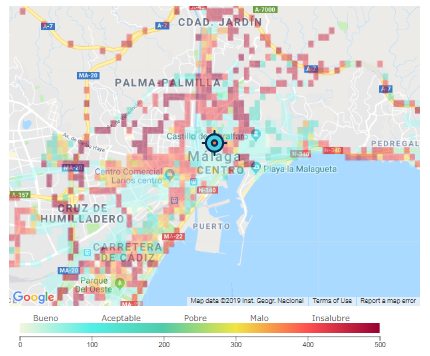
\includegraphics[width=12cm]{myLocation}
    \caption{My Location}
\end{figure}

Regarding flexibility, the user can see the situation of the air pollution by dates. Filtering in the area
intermediate, can be done both by medical conditions and by contamientes agents. Finally, in the lower area where we have
the historical by area and personalized, we can visualize the information with different granularity, time, day, month and year and we can also
select the date we want.

\begin{figure}[ht]
    \centering
   \subfigure[Date filter]
    {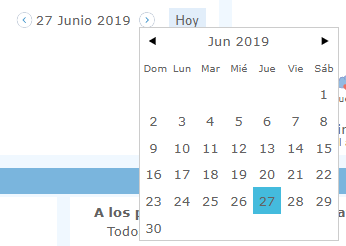
\includegraphics[width=5.5cm  ]{dateFilter}}
    \hfill
    \subfigure [Medical conditions filter]
       { \includegraphics[width=5.5cm]{MedicalConditionFilter}}
    \vfill
     \subfigure[Pollutans filter]
     { \centering 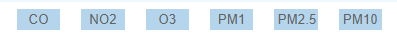
\includegraphics[width=6cm]{pollutansFilter}}
  
  \caption{Filters}
    \end{figure}
    The same style, colors and iconography are used throughout the design so that the user can get familiar quickly and can
    Pay attention to the meaning of the data instead of getting lost in the design and trying to find its meaning.
    
    Due to the large amount of data that is offered to the user, a waiting wheel has been implemented to indicate
    that the tool is processing information. Each time a control is pressed on the page, it is indicated with a change
    of tonality. Also progressive transitions are used, when the graphics have to represent new information it does not
    at once, as this could produce a guide that can be interpreted as an error on the part of the user.
    
    \begin{figure}[ht]
        \centering
    
        \caption{Waiting symbol}
    \end{figure}
    
    \begin{figure}[ht]
        \centering
       \subfigure[Searching bar]
        {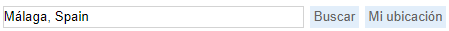
\includegraphics[width=5.5cm  ]{searchingBar}}
        \hfill
        \subfigure [Tabs]
           { 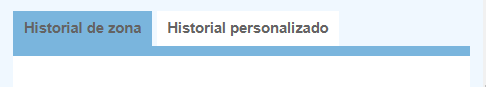
\includegraphics[width=5.5cm]{tabs}}
        \vfill
         \subfigure[Link]
         { 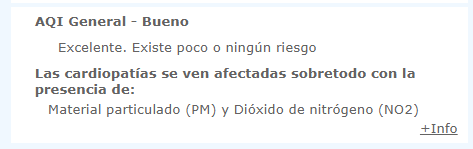
\includegraphics[width=6cm]{link}}
         \hfill
         \subfigure [Waiting symbol]
            { 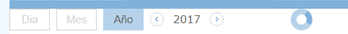
\includegraphics[width=5.5cm]{waitingSymbol}}
      
      \caption{Standard widgets}
        \end{figure}

        The elements that give us familiarity are the iconography that we use to show the AQI. We use clouds, by representation
             of the air, the environment, it is accompanied by a heart if the quality is good, of a symbol of exclamation if it is poor, of a cross if it is
             bad and we change to a gas mask if the state is unhealthy.
            
             Today we are all used to GoogleMaps maps, so it has been integrated to represent the map and not another,
             since users are familiar with how they look and how they are used.      





\elsparagraph{Evaluation}  
\begin{itemize}
    \done Has a relaxed aesthetic where graphics with information prevail
   \done The representation follows a sequence logic
    \done Familiarity, repetition of structures and colors that represent the same and respect standards
    \done Flexibility. The user can make multiple selections
    \crossed Waiting times should be improved
    
\end{itemize}
\newpage